Na základě shromážděných požadavků na aplikaci v částech \ref{section:pozadavky} a \ref{section:pozadavkyCele} byl sestaven obecný model kritických částí aplikace. Základem volební aplikace je samozřejmě model hlasování. Entita \phpinline{Election} představuje kořen stejnojmeného agregátu (\it{Aggregate Root}). Vazby mezi jednotlivými entitami jsou znázorněny jako diagram modelu v obrázku \ref{fig:ElectionModel}. Jednotlivými entitami tohoto agregátu jsou: 
\begin{itemize}
	\item \textbf{Election} - kořen agregátu představující jedny konkrétní volby / hlasování.
	\item \textbf{Question} - ve volbách představuje volenou pozici, v obecném hlasování jednu otázku.
	\item \textbf{Answer} - množina kandidátů, resp. odpovědí na otázku.
	\item \textbf{Voter} - zahrnuje všechny oprávněné voliče.
	\item \textbf{Ballot} - všechny odevzdané hlasovací lístky v daných volbách / hlasování.
\end{itemize}

\begin{figure}[h]
	\centering
	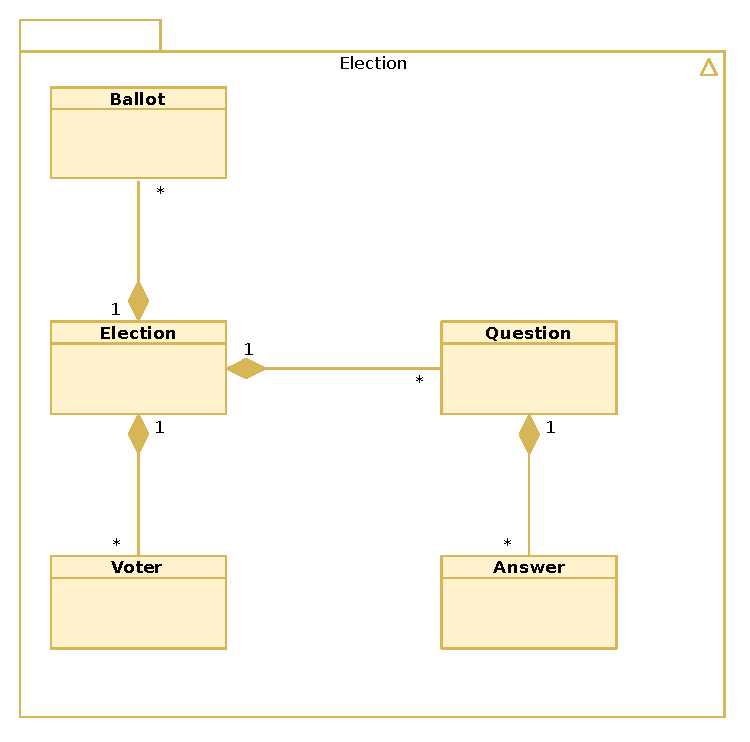
\includegraphics[width=0.6\linewidth]{svg/ElectionModelFull.eps}
	\captionsetup{width=0.6\linewidth}
	\caption[Model objektů balíčku Election]{Model objektů balíčku Election (zdroj: vlastní)}
	\label{fig:ElectionModel}
\end{figure}

Druhou zásadní částí aplikace je systém pro správu přístupu uživatelů (ACL). Nejjednodušší implementací takového systému je přiřazení oprávnění pomocí statické konfigurace. Tento přístup podporuje Nette bez nutnosti jakéhokoli dalšího rozšiřování o vlastní správu oprávnění. Nicméně takový přístup značně limituje flexibilitu aplikace, jelikož se jakákoli změna musí ručně zapsat do konfigurace, která bývá většinou uložena na serveru ve formě souboru. Z tohoto důvodu byl namodelován vlastní ACL systém.

\begin{figure}[h]
	\centering
	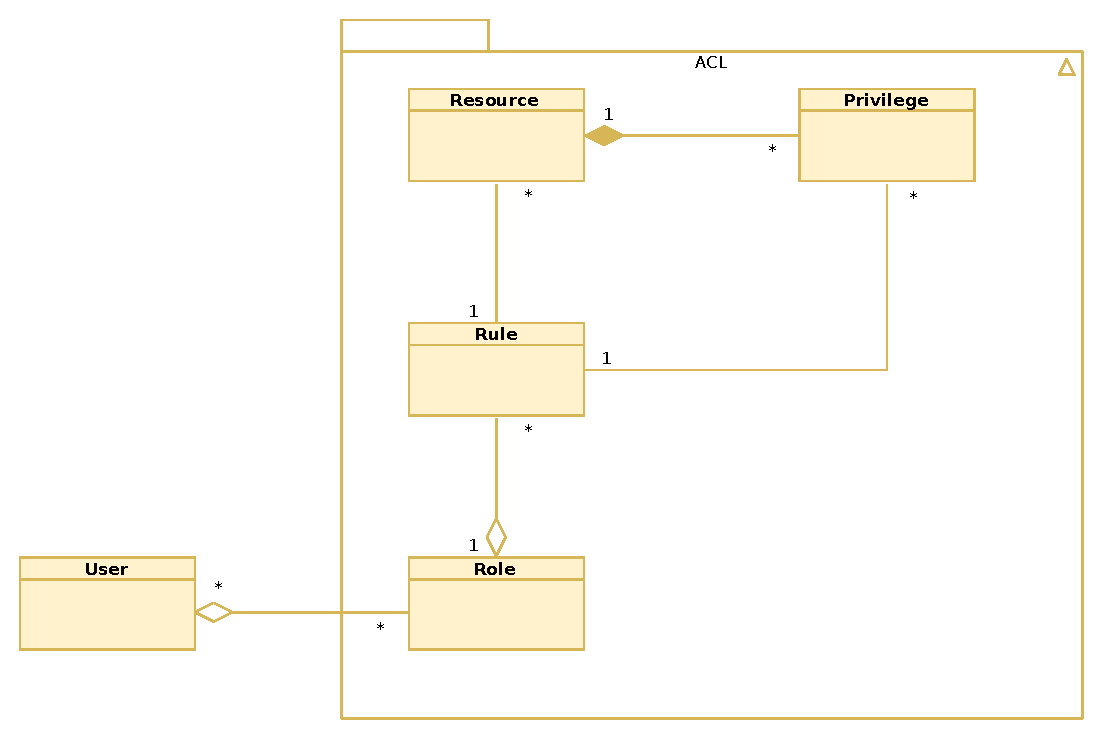
\includegraphics[width=\linewidth]{svg/ACLModelFull.eps}
	\captionsetup{width=\linewidth}
	\caption[Model objektů balíčku ACL]{Model objektů balíčku ACL (zdroj: vlastní)}
	\label{fig:AclModel}
\end{figure}
V tomto případě je kořenem agregátu entita \phpinline{Role} symbolizující jednu roli uživatele. Role může mít nastavena pravidla \phpinline{Rule}, která budou řídit přístup k~prostředkům \phpinline{Resource} a akcím \phpinline{Privilege} na nich vykonávaných. Každé pravidlo je kombinací právě jednoho prostředku a jedné akce. Pravidlo zároveň určuje, jestli je pro danou roli tato akce povolena nebo zakázána (\it{allow / deny}). Tabulka \ref{tab:prikladyACL} ukazuje příklady možného nastavení tohoto systému.


% \tab{popisek}{label}{rozměr (0.0 - 1.0)}{definice sloupců}{obsah} 
\tab{Příklady nastavení ACL}{tab:prikladyACL}{1}{llll}{
	\hline
	Role & Prostředek & Akce & Pravidlo \\
	\hline
	Student			&		Election		&		View		&	allow		\\
	Student			&		Election		&		Vote		&	allow		\\
	Student			&		Election		&		Delete	&	\bf{deny}\\
	Komise			&		Election		&		Count		&	allow		\\
	Administrator	&		Election		&		Activate	&	allow		\\
	SuperAdmin		&		User			&		Create	&	allow		\\
	\hline
}
\clearpage
